%************************************************
% Implementierung
%************************************************
\chapter{Implementierung}
\label{sec:implementation}

\TODO{}

\section{Objektstruktur}
\label{sec:implementation:structure}

\TODO{} wurde zunächst eine Objektorientierte Datenstruktur erarbeitet, die eine Welt repräsentieren und Operationen auf der Welt durchführen kann. \figreft{fig:implementation:program:uml} zeigt ein UML-Diagram dieser Struktur. Zur besseren Übersicht wurde diese Darstellung auf die wehsentlichen zum Verständnis notwenigen Klassen, Attribute und Operationen beschränkt.

\begin{figure}
  \begin{tikzpicture}
    \tikzstyle{every node}=[font=\small]

    \begin{class}[text width=5cm]{World}{4.75,0}
      \attribute{commands}
      \attribute{sensors}

      \operation{command(command: Command)}
      \operation{sensor(sensor: Sensor): boolean}
    \end{class}

    \begin{class}[text width=3cm]{Size}{-1.5,-1}
      \attribute{width: number}
      \attribute{height: number}
    \end{class}

    \begin{class}[text width=3cm]{WorldState}{11,-1.5}
      \attribute{step: number}
      \attribute{time: number}
      \attribute{prev: WorldState}
    \end{class}

    \begin{class}[text width=4cm]{Tile}{-1,-3.5}
      \attribute{position: Position}
      \attribute{freightTarget: Freight}

      \operation{addFreight(freight: Freight)}
      \operation{removeFreight(): Freight}
    \end{class}

    \begin{class}[text width=5cm]{Truck}{10,-5}
      \attribute{position: Position}
      \attribute{facing: number}

      \operation{loadFreight(freight: Freight)}
      \operation{unloadFreight(): Freight}
      \operation{turn(turnDirection: TurnDirection)}
      \operation{move()}
    \end{class}

    \begin{class}[text width=6cm]{TrafficLight}{4.75,-10}
      \attribute{redPhase: number}
      \attribute{greenPhase: number}
      \attribute{initial: number}

      \operation{isRed(step: number): boolean}
      \operation{isGreen(step: number): boolean}
    \end{class}

    \begin{enumeration}[text width=4cm]{TileOpening}{-1,-8}
      \attribute{None}
      \attribute{North}
      \attribute{East}
      \attribute{South}
      \attribute{West}
    \end{enumeration}

    \begin{enumeration}[text width=3.5cm]{Freight}{4.25,-4.5}
      \attribute{Red}
      \attribute{Green}
      \attribute{Blue}
    \end{enumeration}

    \begin{enumeration}[text width=4cm]{TurnDirection}{10.5,-10.5}
      \attribute{Straight}
      \attribute{Left}
      \attribute{Right}
    \end{enumeration}

    \aggregation{World}{size}{1}{Size}
    \aggregation{World}{states}{*}{WorldState}
    \aggregation{WorldState}{tiles}{*}{Tile}
    \aggregation{WorldState}{truck}{1}{Truck}
    \aggregation{Tile}{trafficLights}{0..4}{TrafficLight}
    \unidirectionalAssociation{Truck}{turning}{1}{TurnDirection}
    \unidirectionalAssociation{Tile}{openings}{1..4}{TileOpening}
    \unidirectionalAssociation{Truck}{freight}{0..*}{Freight}
    \unidirectionalAssociation{Tile}{freight}{0..*}{Freight}
  \end{tikzpicture}
  \caption{Vereinfachtes UML-Diagramm der Weltobjektstruktur}
  \label{fig:implementation:program:uml}
\end{figure}

Wurzelelement dieser Struktur ist die \inlinec{World}-Klasse. Sie wird mit einer Beschreibung (\inlinec{WorldDescription}) der zu genrierenden Welt instanziiert. Anhand dieser Beschreibung erzeugt der Kontruktor die Größe (\inlinec{Size}) der Welt, einen Lastwagen (\inlinec{Truck}) und eine Menge von Kacheln (\inlinec{Tile}). Lastwagen und Kacheln werden in einen Weltzustand (\inlinec{WorldState}) verpackt. Die Daten eines einmal gespeicherten Zustandes werden nicht mehr geändert. Stattdessen wird eine Kopie des aktuellen Zustandes erzeugt, verändert und in die Liste aller Zustände abgespeichert. Dieses Vorgehen wurde gewählt, um dem Nutzer zu ermöglichen Aktionen wieder rückgängig zu machen. Außerdem vereinfacht sie die für die Animationen \TODO{Verweis} notwenige Interpolation zwischen Zuständen. Die Veränderung der Zustände übernimmt die \inlinec{World}-Klasse in der Operation \inlinec{command}.

\section{Programmiersprache}

Elemente der Sprache

\begin{itemize}
  \item Wichtigster Bestandteil sind die \emph{atomaren Befehle}. Durch die Aneinanderreihung mehrerer Befehle lässt sich bereits ein sinnvolles Programm implementieren. Als notwendige Befehle wurden identifiziert:
  \begin{itemize}
    \item \emph{Vorwärts fahren}: Bewegt den Lastwagen nach Vorne. Falls dabei ein Blinker in eine Richtung gesetzt ist, biegt der Laswagen in die entsprechende Richtung ab.
    \item \emph{Blinker links setzten}: Setzt den Blinker auf der linken Seite. Dadurch biegt der Lastwagen bei der nächsten Vorwärtsbewegung links ab.
    \item \emph{Blinker rechts setzten}: Setzt den Blinker auf der rechten Seite. Bei der nächsten Vorwärtsbewegung biegt der biegt der Lastwagen dadurch entsprechend rechts ab.
    \item \emph{Blinker ausschalten}: Schaltet einen vorher eingeschalteten Blinker wieder aus.
    \item \emph{Aufladen}: Läd ein Frachstück, welches vor dem Lastwagen liegt auf.
    \item \emph{Abladen}: Läd ein Frachtstück auf eine Ablagefläche oder einen leeren Steckenabschnitt vor dem Lastwagen wieder ab.
    \item \emph{Warten}: Wartet einen Zeitschritt ab. Dieser Befehl ist wichtig um das warten auf eine Ampel zu ermöglichen.
  \end{itemize}
  \item Um Codeverdoppelung zu vermeiden kann eine \emph{Schleife} eingesetzt werden, die einen Befehlsblock wiederholt. Die Anzahl der Wiederholungen kann vom Nutzer festgelegt werden.
  \item Um Verzweigungen Nutzen zu können, gibt es die Möglichkeit Werte von \emph{Sensoren} abzufragen. Sensoren stehen immer entweder auf Wahr oder Falsch. Folgende Sensoren stehen zur Verfügung:
  \begin{itemize}
    \item \emph{Ampel ist rot}: Dieser Sensor ist Wahr, wenn die Ampel vor dem Lastwagen rot ist. Ist, die Ampel grün, oder es gibt keine Ampel vor dem Lastwagen, so steht dieser Sensor auf Falsch.
    \item \emph{Ampel ist grün}: Ananlog dazu, ist dieser Sensor Wahr, wenn die Ampel vor dem Lastwagen grün ist und Falsch, wenn sie auf rot steht oder es keine Ampel vor dem Lastwagen gibt.
    \item \emph{Kann geradeaus fahren}: Dieser Sensor wertet zu Wahr aus, wenn das Straßennetz es zulässt, dass der Lastwagen im nächsten Schritt geradeaus fahren kann.
    \item \emph{Kann links abbiegen}: Dieser Sensor wertet zu Wahr aus, wenn im nächsten Schritt links abgebogen werden kann.
    \item \emph{Kann rechts abbiegen}: Wenn im nächsten Schritt nach rechts abgebogen werden kann, wertet dieser Sensor zu Wahr aus.
    \item \emph{Ist gelöst}: Wenn die aktuelle Welt gelöst wurde, also alle Frachtstücke zu ihren Zielen transporiert wurden, wertet dieser Sensor zu Wahr aus.
  \end{itemize}
  \item Mit den Sensoren ist es möglich eine \emph{Schleife mit Abbruchbedingung} zu nutzen. Diese wiederholt den Befehlsblock solange bis der angegebene Ausdruck zu Wahr auswertet.
  \item Sensoren ermöglichen außerdem \emph{Verzweigungen}, die einen Befehlsblock nur dann ausführen, wenn der angegebene Sensor zu Wahr ausgewertet wird.
  \item Es ist möglich den Wert von Sensoren zu \emph{negieren}.
  \item Mit Hilfe von \emph{Verknüfungen} mit "und" und "oder", können neue Ausdrücke erzeugt werden, welche wiederum in Schleifen und Verzweigungen verwendet werden können. So ist es z.B. möglich zu prüfen, ob das vorrausliegende Steckenstück eine Kurve ist: (Kann nicht geradeaus fahren und ((Kann links abbiegen und Kann nicht rechts abbiegen) oder (Kann nicht links abbiegen und Kann rechts abbiegen)))
  \item Desweiteren ist es möglich eigene \emph{Prozeduren} zu definieren und aufzurufen. Dies ermöglicht zusätzlich die Nutzung von Rekursion.
\end{itemize}

\subsection{Auswertung}

Für die Auswertung und Ausführung des durch den Syntaxbaum beschriebenen Code kommen zwei Vorgehensweisen infrage. Im Grundlagenkapitel \ref{sec:basics:compile-interpret} wurde der Unterschied zwischen Kompilieren und Interpretieren im klassischen Sinne bereits erklärt. Da im Browser jedoch nicht direkt Maschienencode ausgeführt werden kann ist der Unterschied in diesem Zusammenhang etwas anders zu verstehen.

\begin{itemize}
  \item Beim \emph{Interpretieren} wird der Syntaxbaum nach und nach durch ein in JavaScript geschriebenes Programm abgearbeitet und die entsprechenden Befehle direkt ausgeführt. In dieser Umgebung lässt sich der Fortschritt des Programms leicht verfolgen, da der Interpreter zu jedem Zeitpunkt die Position kennt bis zu der der Code bisher ausgeführt wurde. Dies ermöglicht den Einbau von Aussagekräftigen Debuggingfunktionen für den den auszuführenden Code.
  \item Im Unterschied dazu ist \emph{Kompilieren} in diesem Zusammenhang so zu verstehen, dass ein JavaScript-Programm den Syntaxbaum zunächst in einen vollständig ausführbaren JavaScript-Code überführt. Der JavaScript-Code liegt bei diesem Vorgehen nach dem Kompilieren als String vor und kann anschließend als ganzes in einer Art Sandkasten ausgeführt werden. Innerhalb dieser "Blackbox" lässt sich nur recht unzuverlässig auf den aktuellen Zustand des laufenden Programmes schließen ohne zusätzlichen Code code einzufügen, der die Lesbarkeit des generierten Codes verschlechtert. Eben diese Lesbarkeit des generierten Codes ist einer der wichtigsten Vortile dieser Vorgehensweise. Der Code lässt sich nicht nur für seine Ausführung nutzen, sondern kann gerade im Kontext einer Lernsoftware für den Nutzer interessant sein.
\end{itemize}

Im Verlauf der Arbeit wurde die Vorgehensweise "Kompilieren" an dieser Stelle als Anforderung festgelegt, da dieses Vorgehen speziell für BlattWerkzeug den Vorteil mit sich bringt, dass generierter Code in Zukunft vor der Ausführung noch vom Nutzer angesehen und bearbeitet werden kann, was den Übergang zu einer Universalsprache erleichtern würde \TODO{Verweis auf Ausblick}.

Für die Kompilierung des Syntaxbaum wird auf den von BlattWerkzeug zur Verfügung gestellten Codegenerator-Strukturen zurückgegriffen, die es ermöglichen einen Codegenrator zu implementieren, der Übersetzungsregeln für jeden Knotentypen definiert. \figreft{fig:implementation:program:evaluation:while} zeigt die Implementierung eines Codegenrators für Knoten, die eine While-Schleife repräsentieren. Zwischen den Klammern innerhalb der \inlinec{while}-Anweisung wird der Kindknoten für die Bedingung der Schleife eingefügt, gefolgt vom Inhalt der Schleife. Diese Kindknoten werden wiederrum durch ähnlich aufgebaute Generatoren umgewandelt bis der Vollständige Code des Wurzelknoten im Syntaxbaum generiert wurde.

\begin{figure}
  \begin{lstlisting}
    {
      type: {
        languageName: "trucklino_program",
        typeName: "loopWhile"
      },
      converter: {
        init: function(node: Node, process: CodeGeneratorProcess<State>) {
          process.addConvertedFragment(`while (`, node);
          node.getChildrenInCategory('pred').forEach((c) => process.generateNode(c));
          process.addConvertedFragment(`) {`, node, OutputSeparator.NEW_LINE_AFTER);
          process.indent(() => {
            node.getChildrenInCategory('body').forEach((c) => process.generateNode(c));
          });
          process.addConvertedFragment(`}`, node, OutputSeparator.NEW_LINE_AFTER);
        }
      }
    }
  \end{lstlisting}
  \caption{Beispielhafte Implementierung eines Codegenrator für eine While-Schleife}
  \label{fig:implementation:program:evaluation:while}
\end{figure}

Dem kompilierten Code muss zur Ausführung eine Umgebung bereitgestellt werden, welche die eingangs als "atomaren Befehele" bezeichneten Funktionen, sowie Funktionen zur Ermittlung der Sensorwerte zur Verfügung stellt. Für diese Aufgabe bietet sich der \inlinec{Function}-Konstruktor\footnote{\url{https://developer.mozilla.org/de/docs/Web/JavaScript/Reference/Global_Objects/Function}} an. Im Gegensatz zu \inlinec{eval} ermöglicht der \inlinec{Function}-Konstruktor die Ausführung von Code im globalen Gültigkeitsbereich, was zu besseren Programmiergewohnheiten führt und eine effizientere Code-Minimierung ermöglicht \cite{mdn-function}. In diesem speziellen Fall wird für die Ausfühung des Codes der \inlinec{AsyncFunction}-Konstruktor verwendet (siehe dazu \TODO{Verweis Animation}).

Für die Bereitstellung der Befehle und Sensoren werden im Folgenden drei Varianten betrachtet, die in \TODO{Verweis auf Abbildung}:

\begin{enumerate}
  \item Eine Enum-Klasse mit allen Sensoren und Befehlen, sowie zwei Funktionen deren Auswertung, gibt es schon. Darauf aufbauend wäre eine naheliegend Möglichkeit, diese Funktionen in der Welt bereitzustellen. Ein deutlicher Vorteil dieser Lösung ist der geringe zusätzliche Implementierungsaufwand und die verbesserte Wartbarkeit. Kommen neue Befehle oder Sensoren dazu, stehen diese automatisch auch in der Umgebung zur Verfügung. Der generierte Code ist jedoch nicht intuitiv und sollte er dem Nutzer angezeigt werden, nicht besonders gut zu verstehen. Außerdem halten sich die Funktionsaufrufe nicht an gängige Muster, was den späteren Umstieg auf Universalsprachen erschweren könnte. \TODO{Verweis auf Grafik}
  \item Eine weitere Möglichkeit \TODO{this}
  \item \TODO{Parameter}
\end{enumerate}

\begin{figure}
  \begin{subfigure}[b]{\textwidth}
    \begin{lstlisting}
      let code = `
        functions.goIfGreen = function() {
          if (sensor(Sensor.lightIsGreen)) {
            command(Command.goForward);
          }
        }
        functions.goIfGreen();
      `;
      let f = new Function('functions', 'sensor', 'Sensor', 'command', 'Command', code);
      f({}, (s) => world.sensor(s), Sensor, (c) => world.command(c), Command);
    \end{lstlisting}
    \caption{Code für ein Quadrat}
    \label{fig:implementation:code:func}
  \end{subfigure}
  \begin{subfigure}[b]{\textwidth}
    \begin{lstlisting}
      let code = `
        this.goIfGreen = () => {
          if (this.lightIsGreen()) {
            this.goForward();
          }
        }
      `;
      let f = new Function(code);
      f.call({
        goForward: () => world.command(Command.goForward),
        ...
        
        lightIsGreen: () => world.sensor(Sensor.lightIsGreen),
        ...
      });
    \end{lstlisting}
    \caption{Code für ein Dreieck}
    \label{fig:implementation:code:this}
  \end{subfigure}
  \begin{subfigure}[b]{\textwidth}
    \begin{lstlisting}
      let code = `
        function goIfGreen() {
          if (lightIsGreen()) {
            goForward();
          }
        }
        goIfGreen();
      `;
      let f = new Function('goForward', ..., 'lightIsGreen', ..., code);
      f(
        () => world.command(Command.goForward),
        ...
        () => world.sensor(Sensor.lightIsGreen),
        ...
      );
    \end{lstlisting}
    \caption{Code für ein Haus}
    \label{fig:implementation:code:param}
  \end{subfigure}
  \caption{Zeichnen eines Hauses in LOGO}
  \label{fig:implementation:code}
\end{figure}

- Funktionen und Sensoren aufrufen, verschiedene Möglichkeiten:
    - Eine Funktion für Befehle, eine Funktion für Sensoren und gewünschten Befehl/Sensor als Konstante. Vorteil: Sehr gute Wartbarkeit, da Befehle nur an einer Stelle hinzugefügt werden müssen. Nachteil: Unintuitiver generierter Code / Anders als "übliche" Schreibweise
    - Funktionen und Befehle werden im Kontext übergeben und über this aufgerufen. Vorteil: Gute wartbarkeit (wenn auch doppelte Pflege notwendig), Codelesbarkeit gut, Einfache übergabe im Objekt. Nachteil: Vor jeder Funktion/Sensor muss ein this stehen
    - Funktionen und Befehle werden als Parameter übergeben. Vorteil: Direkter Aufruf der Funktionen ohne zusätzlichen Code dadurch sehr gute Codelesbarkeit. Nachteil: Unübersichliche Definition der Funktion und dadurch schlechtere Wartbarkeit.

- Behandlung von Endlosschleifen

\section{Darstellung}

\subsection{Technologie}

Also mögliche Technologien für die Darstellung und Animation der Welt im Browser wurden im vier Ansätze evaluiert.

\begin{itemize}
  \item Rendering über klassische \emph{HTML}-Elemente und Styling mittels CSS und Integration von nachgeladenen Bilddateien.
  \item Rendering mittels eines eingebetteten \emph{SVG}-Element.
  \item Rendering mittels eines \emph{Canvas}-Element und Integration von nachgeladenen Bilddateien.
  \item Einsatz von \emph{WebGL} für die Darstellung einer dreidimensionalen Welt.
\end{itemize}

WebGL ist als Technologie für diese Arbeit als zu mächtig einzustufen. Die Erstellung von dreidimensionalen Modellen hätte den Rahmen dieser Arbeit gesprengt und im Vergleich zu den übrigen Technologien keinen nennenswerten Nutzen gehabt.

Rendering mittels HTML und SVG haben den Vorteil, dass sie sehr von den Funktionen des Angular-Framework profitieren. Die Datenstruktur kann direkt an HTML-Elemente angebunden werden und Angular kümmert sich um die Aktualisierung des DOM. Dieses Vorgehen reduziert den Aufwand für die Implementierung des Renderes enorm. Zusätzlich bringt Angular nativ ein Animationsframework mit. Für die Implementierung eines Prototyp wurde das Rendering mittels eines SVG-Element gewählt, da es gegenüber einfachem HTML den Vorteil bietet, Grafiken direkt und ohne zusätliches Nachladen von Ressourcen integrieren zu können.

In der Implementierung des Prototyp erwies sich aber genau dieses Animationsframework als ein Nachteil dieser Technologie. Angular setzt an dieser Stelle auf ein Zustandsbasiertes System. Eine Animationen finden immer zwischen definierten Zuständen statt. Zustände können bestimmte CSS Regeln definieren, zwischen denen bei einem Zustandswechel interpoliert wird \cite{angular-animations}. Dieses System ist mit den Anforderungen, die der im Rahmen dieser Arbeit behandelte Anwendungsfall stellt nicht kompatibel. Für die Animation eines Lastwagen müsste vielmehr zwischen verschiedenen Positionen interpoliert werden. Diese lassen sich nicht sinnvoll auf Zustände abbilden.

So setzt die aktuelle Version des Programms auf einen Renderer mittels Canvas-Element. Dass Angular keine Funktionen zum Rendern in einem Canvas-Element bereithält und dieser Prozess vollständig außerhalb und unabhängig von Angular stattfinden muss, erwies sich schnell als Vorteil. Der Renderer hat dadurch keine externen Abhängigkeiten, ermöglicht eine leichte Integration in BlattWerkzeug und könnte potenziell auch in eine Anwendung portiert werden, welche Angular nicht einsetzt.

\subsection{Objektstruktur}

Die Objektstruktur des Renderers ist in \figreft{fig:implementation:rendering:uml} zur besseren Übersicht vereinfacht dargestellt. Wurzelklasse ist hier der Renderer, welche mit einem \inlinec{World}-Objekt (Die Objektstruktur wurde in Abschnitt \ref{sec:implementation:structure} beschrieben) und einem Canvas-Context instanziiert wird. Mit dem Aufruf der \inlinec{render}-Methode wird der Render-Prozess gestartet. Diese Methode zeichnet den Canvas-Inhalt und ruft sich mittels der \inlinec{requestAnimationFrame}-Funktion\footnote{\url{https://developer.mozilla.org/en-US/docs/Web/API/window/requestAnimationFrame}} immer wieder selbst auf.

Die Eigentliche Zeichenaufgabe gibt die \inlinec{Renderer}-Klasse jedoch an einen Baum von \inlinec{ObjectRenderer}-Klassen ab, die für die Darstellung wehsentlicher visueller Objekte zuständig sind. Die Struktur der \inlinec{ObjectRenderer} ist an der Weltobjektstruktur \tref{sec:implementation:structure} orientiert. Die \inlinec{Renderer}-Klasse hält eine Instanz eines \inlinec{WorldRenderer}, welcher die von ihm gehaltene \inlinec{WorldStateRenderer}-Instanz über Zustandsänderungen der Welt informiert. Der \inlinec{WorldStateRenderer} verwaltet genau eine \inlinec{TruckRenderer}-Instanz, welche für das letztendliche Zeichnen des Lastwagen und die Animation von dessen Zustandsübergängen verantwortlich ist, sowie die notwenige Anzahl von \inlinec{TileRenderer}-Instanzen. Die \inlinec{draw}-Methode der \inlinec{ObjectRenderer} werden immer mit einem \inlinec{RenderingContext} aufgerufen, welcher den Zeitstempel der Animation verwaltet, einen Verweis auf den zu verwendenden Canvas-Context enhält, sowie einige Hilfsmethoden zum Zeichnen auf demselbigen bereitstellt.

Das sichtbare Bild wird durch die ObjectRenderer vollständig aus verschiedenen Komponenten zusammengesetzt, die aus SVG-Sprites an die richtige Stelle im Bild gezeichnet werden. Die Hintergründe der Straßen stammen aus einer freien Sammlung von Spielegrafiken\footnote{\url{https://opengameart.org/node/16589}}, der Truck und die Fracht wurden für den Zweck dieser Arbeit selbst gezeichnet. Alle 16 Varianten von Kacheln sind im Sprite verfügbar. Lediglich der Truck muss vor dem Zeichnen in die richtige Richtung gedreht werden. Ein Vorbereiten aller möglichen Drehungen des Lastwagen im Sprite ist an dieser Stelle nicht sinnvoll, da die Drehung des Lastwagen animiert interpoliert werden soll.

\begin{figure}
  \begin{tikzpicture}
    \tikzstyle{every node}=[font=\small]

    \begin{class}[text width=7cm]{Renderer}{1,0}
      \attribute{running: boolean}

      \operation{constructor(world: World, ctx: CanvasContext)}
      \operation{stop()}
      \operation{render(timestamp: TimeStamp)}
    \end{class}

    \begin{class}[text width=5cm]{RenderingContext}{9,0}
      \attribute{ctx: CanvasRenderingContext2D}
      \attribute{width: number}
      \attribute{height: number}
      \attribute{start: TimeStamp}
      \attribute{previousFrame: TimeStamp}
      \attribute{currentFrame: TimeStamp}

      \operation{animationSpeed(): number}
    \end{class}

    \begin{interface}[text width=5cm]{ObjectRenderer}{3.5,-3}
      \operation{draw(ctx: RenderingContext)}
    \end{interface}

    \begin{class}[text width=3cm]{WorldRenderer}{-1,-5}
      \implement{ObjectRenderer}

      \attribute{world: World}

    \end{class}

    \begin{class}[text width=4cm]{WorldStateRenderer}{-0.5,-7.5}
      \implement{ObjectRenderer}

      \attribute{state: WorldState}
      \attribute{freightTarget: Freight}

      \operation{update(state: WorldState)}
    \end{class}

    \begin{class}[text width=2.75cm]{TileRenderer}{5.5,-6}
      \implement{ObjectRenderer}

      \attribute{tile: Tile}

      \operation{update(tile: Tile)}
    \end{class}

    \begin{class}[text width=3.5cm]{TruckRenderer}{9.75,-7}
      % \implement{ObjectRenderer}

      \attribute{truck: Truck}
      \attribute{prevTruck: Truck}
      \attribute{initial: number}

      \operation{update(truck: Truck)}
    \end{class}

    \composition{Renderer}{ctx}{1}{RenderingContext}
    \composition{Renderer}{worldRenderer}{1}{WorldRenderer}
    \composition{WorldRenderer}{stateRenderer}{1}{WorldStateRenderer}
    \composition{WorldStateRenderer}{truckRenderer}{1}{TruckRenderer}
    \composition{WorldStateRenderer}{tileRenderers}{0..*}{TileRenderer}

    \draw[umlcd style implement line](ObjectRenderer) -- (TruckRenderer.north);
  \end{tikzpicture}
  \caption{Vereinfachtes UML-Diagramm der Rendererobjektstruktur}
  \label{fig:implementation:rendering:uml}
\end{figure}

Wenn die \inlinec{render}-Methode aus einer Angular-Anwendung heraus aufgerufen wird, empfielt es sich diesen Aufruf außerhalt der Angular-Zone vorzunehemen. Angularanwendungen werden immer innerhalb der "Angular-Zone" ausgeführt. Wenn ein Browserereignis (z.B. ein Klick oder ein \inlinec{setTimeout}) eintritt, wird die Angular Zone betreten und der Code zur Ereignisbehandlung ausgeführt. Anschließend führen die Zone und Angular die Änderungserkennung für die Anwendung durch. In den meisten Fällen ist dieses Verhalten erwünscht. Beim Zeichnen führt dies jedoch dazu, dass \inlinec{requestAnimationFrame} ebenfalls in der Angular-Zone ausgeführt wird. Dies bedeutet, wenn eine Animation läuft, werden pro Sekunde bis zu 60 Änderungserkennungen ausgeführt. \cite{angular-canvas} Da die \inlinec{render}-Methode lediglich der Darstellung dient, keinerlei Änderungen an der Welt oder ihren Zuständen vornimmt und somit nie Änderungen zu detektieren sein werden, kann und muss sie dementsprechend außerhalb der Angular-Zone ausgeführt werden.

\begin{figure}
  \begin{lstlisting}
    ...
    constructor(private ngZone: NgZone) { }

    ngOnInit() {
      this.ngZone.runOutsideAngular(() => this.draw());
    }
    ...
  \end{lstlisting}
  \caption{Aufruf außerhalb der Angular-Zone (in Anlehnung an \cite{angular-canvas})}
  \label{fig:implementation:program:evaluation:while}
\end{figure}

\subsection{Lastwagen-Position}

- Möglichkeit A: Lastwagen halten auf Mitte der Kachel und drehen sich auf der Stelle (ähnlich zu Kara und Lightbot)
  => Lastwagen können auch wenden, aber das Verhalten sieht unnatürlich aus.
- Möglichkeit B: Lastwagen halten auf dem Rand der Kachel und es kann ein Blinker nach links oder rechts gesetzt werden, der die Fahrtrichtung beim nächsten Vorwärtsfahren beeinflusst
  => Verhalten sieht deutlich natürlicher aus und ist näher am Vorbild. Allerdings kann der Lastwagen nun nicht mehr auf der Stelle wenden und muss eventuell längere Strecken fahren.
  => Erste Idee: Pfeil davor anzeigen, Zweite Idee: Blinker
  => Rückwärts fahren?
- Bewegung: Absolut (N, E, S, W) vs. Relativ (Links, Rechts, Geradeaus)

Sowohl bei Kara \TODO{Verweis}, als auch bei Lightbot \TODO{Verweis} bewegt sich die Spielfigur von einer Kachel des Spielfeldes zur nächsten und kommt zwischen den Schritten auf der Mitte der Kachel zum stehen. Eine Drehung findet auf der Stelle statt. Die Spielfigur dreht sich um sich selbst und kann sich so in alle 4 Richtungen bewegen. So liegt es nah diese Verhalten auch für den Lastwagen zu implementieren, jedoch ist zu bedenken, dass die Spielfiguren von Kara und Lightbot sich in einem realen Umfeld anders Bewegen als ein Lastwagen. Wärend eine Drehung auf der Stelle für einen Marienenkäfer und einen hüpfenden Roboter kein Problem darstellen, wäre der Fahrer eines Lastwagens mit dieser Aufgabe wohl überfordert. Ein Lastwagen dreht sich nur dann, wenn bei einer Vorwärtsbewegung die Lenkung eingeschlagen wird. Um dieses Verhalten auch in die Mikrowelt zu übertragen, wurde eine Implementierung gewählt, bei der der Lastwagen auf der Kante der Kachel zum stehen kommt. An dieser Stelle hat der Spieler die Möglichkeit einen Blinker nach rechts oder links zu setzten und damit die Richtung bei der nächsten Vorwärtsbewegung zu beeinflussen \TODO{Verweis auf Grafik}. Im Gegensatz zur erstgenannten Methode ist mit diesem Ansatz kein Wenden möglich. Der Lastwagn muss eventuell einen Umweg fahren um sein Ziel zu erreichen und darf sich in keine Sackgassen begebn. Für die Zukunft wäre es allerdings denkbar, einen Rückwärtsgang einzuführen \TODO{Verweis auf Ausblick}.

- Nebeneffekt: Richtiges Verhalten an Ampeln

\begin{figure}
  \begin{subfigure}[b]{0.45\textwidth}
    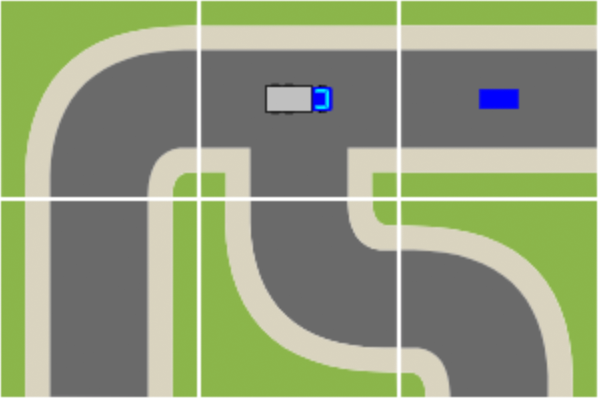
\includegraphics[width=\textwidth]{gfx/implementation-rendering-truck-A.png}
    \caption{Haltepunkt auf der Mitte der Kachel}
    \label{fig:implementation:rendering:truck:a}
  \end{subfigure}\hfill
  \begin{subfigure}[b]{0.45\textwidth}
    \includegraphics[width=\textwidth]{gfx/implementation-rendering-truck-B.png}
    \caption{Haltepunkt auf der Kante der Kachel}
    \label{fig:implementation:rendering:truck:b}
  \end{subfigure}\hfill
  \caption{Haltepunkte des Lastwagen im Spielfeld}
  \label{fig:implementation:rendering:truck}
\end{figure}

\subsection{Animationsschritte}

- Neuer Zustand für jede Operation
- Zustände haben unterschiedliche Zeitwerte: Blinker setzen kostet keine Zeit,
  geradeaus fahren oder warten kostet einen Zeitschritt
- Zeitschritte sind besonders für die Berechnung der Ampelstellung relevant
- Position des Lastwagen wird schrittweise interpoliert

- Schitte haben eine feste Zeit, die aber übersprungen wird, wenn ein neuer
  Schritt vor ablauf der Zeit dazu kommt. Dadurch kann ein Programm auch im
  "Schnelldurchlauf" abgespielt werden.

- Kompilieren in JS-Code mit async await
- new AsyncFunction (TypeScript-Compiler-Problem, Anforderung an den Browser)

\section{Integration}

Um mit möglichst wenigen Abhängigkeiten und dadurch der Möglichkeit mit geringerem Zeitaufwand verschiedene Ansätze ausprobieren zu können, wurde zunächst mit der Entwicklung eines Prototypen auf einer "grünen Wiese" begonnen. Auch wenn der Prototyp als Angular-Anwendung aufgesetzt wurde, erfolgte der Großteil der Entwicklung erfolge außerhalb dieser Umgebung. Nachdem der ursprüngliche Ansatz der Darstellung mittels SVG-Grafiken verworfen wurde und die Darstellung auf Canvas-Rendering umgestellt wurde, sind die Objektstruktur, sowie der Renderer wurden völlig unabhängig von Angular, da sie von den von Angular bereitgestellten Strukturen nicht profitieren können. Diese Klassen konnten so ohne Anpassungen in die Umgebung von BlattWerkzeug übernommen werden. Lediglich die rudimentäre Benutzeroberfläche des Prototypen \TODO{Screenshot Prototyp} wurde mit Hilfe von Angular umgesetzt, für die Integration in BlattWerkzeug jedoch nicht mehr benötigt.

\subsection{Angular-Service}

- Auslagerung der Welt in einen Service

\subsection{Fortschrittsmeldungen}

- Rückmeldung über den Fortschritt des Programm zur Anzeige im Drag \& Drop-Editor => Ausblick?
